\clearpage
\noindent\makebox[0pt][l]{\fontsize{13}{16}\selectfont 478}\hfill{\small\textbf{POSTHUMOUS PAPERS.}}\hfill\null\par
\vspace*{32mm}
\begin{center}
{\Large\bfseries POSTHUMOUS PAPERS.}\par\vspace{15mm}
[1.]\par\medskip
\textbf{Effect of imperfect adjustment of the first heliotrope.}
\end{center}
For greater simplicity, we assume that the axis is horizontal and points
toward azimuth 0, and that the luminous point likewise lies on the horizon at
azimuth $A$. The errors are now of two kinds:

\noindent I. With regard to azimuth.
\begin{list}{}{\setlength{\leftmargin}{9mm}\setlength{\labelwidth}{6mm}\setlength{\itemsep}{2pt}\setlength{\parsep}{0pt}\setlength{\topsep}{3pt}}
\item[1.] If the reticle is too far to the right by $\alpha$,
the light is reflected not to azimuth 0 but to azimuth
$-\alpha$. Thus the effect $=-\alpha$
\item[2.] If the mirror is rotated forward by $\beta$ from its
position perpendicular to the guide rod, the resulting
effect is\hfill $=+2\beta$
\item[3.] If the axis of the sleeve is too far from the telescope
axis, in the ratio $(1+\gamma):1$, the effect is\hfill $=+206265.\gamma.\operatorname{tg}\frac12 A$
\end{list}
\noindent II. With regard to altitude.
\begin{list}{}{\setlength{\leftmargin}{9mm}\setlength{\labelwidth}{6mm}\setlength{\itemsep}{2pt}\setlength{\parsep}{0pt}\setlength{\topsep}{3pt}}
\item[4.] If the mirror is directed upward by $\delta$
(the screw is tightened too much):\hfill $+2\delta\cos\frac12 A$
\item[5.] The bottom of the mirror axis is inclined too far
forward by $\varepsilon$:\hfill $+2\varepsilon\cos\frac12 A^2$
\item[6.] The bottom of the mirror axis is too far to the right by $\zeta$:\hfill $+\zeta\sin A$
\end{list}

\clearpage
\noindent\null\hfill{\small\textbf{HELIOTROPE.}}\hfill\makebox[0pt][r]{\fontsize{13}{16}\selectfont 479}\par\medskip
\begin{list}{}{\setlength{\leftmargin}{9mm}\setlength{\labelwidth}{6mm}\setlength{\itemsep}{2pt}\setlength{\parsep}{0pt}\setlength{\topsep}{0pt}}
\item[7.] The bottom of the telescope axis is too far forward by $\eta$,
but the optical axis can still become parallel to the
principal axis:\hfill $+2\eta\sin\frac12 A^2$
\item[8.] The reticle is too high by $\theta$:\hfill $+\theta$
\end{list}
\noindent One item remains to be added for the azimuth\par
\hspace*{9mm}Effect of parallax $\pi$:\hfill $-\pi\sin A.$
\begin{center}\textbf{For the second heliotrope.}\end{center}
For the azimuth, only the inclination of the two mirrors to one another
comes into consideration. If the small mirror is rotated too far forward by
$\alpha$, the image is reflected toward $-2\alpha$.
\begin{center}
[2.]\par\medskip
\textbf{On adjusting the heliotrope.}
\end{center}
1. An essential requirement for adjusting the heliotrope is a pair of
tripods, at least one of which is adjustable in height, to which one can
easily and accurately give any required difference in height.\ .\ .\ .\ .\ .\ .

2. The simplest way to determine the locus of the reflected image of a
stationary object while the mirror fixed to an axis rotates about that axis
is as follows:

Let $A$ be the intersection of the mirror \textls[120]{surface} with the axis of rotation,
and $B$ a point on the normal to the mirror surface, on the back side of
the mirror, with $AB$ arbitrary. Thus $B$ is fixed relative to the mirror,
but as the mirror rotates it describes a circle in space, in the same sense
as any other point fixed relative to the mirror, for instance the midpoint
of one of the four sides of its rectangular outline. The centre $C$ of that circle lies
on the axis of rotation, and $AC=AB\cos\theta$, where $90^\circ-\theta$ is
the inclination of the mirror to the axis of rotation. The reflected image
$P$ of a point $D$ fixed in space can now be found by drawing through $D$ a
parallel to $AB$ and extending it if necessary until $AP=AD$. The hitherto
arbitrary $AB$ can be taken of such a length that $AC=AE$ when $DE$ is drawn
perpendicular to the axis of rotation $AE$.

\clearpage
\noindent\makebox[0pt][l]{\fontsize{13}{16}\selectfont 480}\hfill{\small\textbf{POSTHUMOUS PAPERS.}}\hfill\null\par
\begin{center}
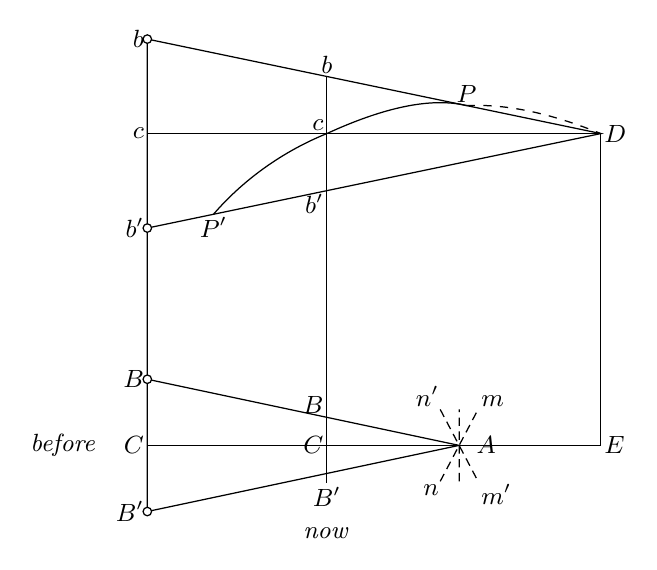
\begin{tikzpicture}[x=12mm,y=12mm,line width=.45pt,every node/.style={font=\small,inner sep=1pt}]
\draw (0,0)--(0,5)--(4.8,4)--(0,3)--cycle;
\draw (0,4)--(4.8,4)--(4.8,.7)--(0,.7);
\draw (0,1.4)--(3.3,.7)--(0,0);
\draw (1.9,4.604)--(1.9,.297);
\draw (.7,3.146) .. controls (1.05,3.55) and (1.48,3.83) .. (1.9,4) .. controls (2.40,4.23) and (2.95,4.40) .. (3.38,4.296);
\draw[dashed] (3.38,4.296) .. controls (3.9,4.32) and (4.4,4.16) .. (4.8,4);
\draw[densely dashed] (3.10,.32)--(3.50,1.08) (3.10,1.08)--(3.50,.32) (3.3,.32)--(3.3,1.08);
\foreach \q in {(0,5),(0,3),(0,1.4),(0,0)} \draw[fill=white] \q circle (.045);
\node[left] at (0,5) {$b$}; \node[left] at (0,4) {$c$};
\node[left] at (0,3) {$b'$}; \node[left] at (0,1.4) {$B$};
\node[left] at (0,.7) {$C$}; \node[left] at (0,0) {$B'$};
\node[above] at (1.9,4.604) {$b$}; \node[above left] at (1.9,4) {$c$};
\node[below left] at (1.9,3.396) {$b'$};
\node[above left] at (1.9,.997) {$B$}; \node[left] at (1.9,.7) {$C$};
\node[below] at (1.9,.297) {$B'$};
\node[above] at (3.38,4.296) {$P$}; \node[below] at (.7,3.146) {$P'$};
\node[right] at (4.8,4) {$D$}; \node[right] at (4.8,.7) {$E$};
\node[right] at (3.45,.7) {$A$};
\node[above left] at (3.12,1.08) {$n'$}; \node[above right] at (3.5,1.08) {$m$};
\node[below left] at (3.12,.32) {$n$}; \node[below right] at (3.5,.32) {$m'$};
\node[left] at (-.5,.7) {\textit{before}};
\node[below] at (1.9,-.14) {\textit{now}};
\end{tikzpicture}
\end{center}
If one then draws $Dc$ parallel to $AC$ and $Cc$ parallel to $ED$, then $Dc=2AC$,
$Ac=AD$, so $c$ lies on the surface of a sphere of radius $AD$ described about
$A$. If one passes a plane through $c$ perpendicular to $Dc$ and in that plane
uses radius $cb=2CB$ to draw about $c$ a circle $bb'$, then $PP'$ lies on the
surface of the right cone with vertex $D$, axis $Dc$, sides $Db$, $Db'$, and
opening angle $bDb'=BAB'=2\theta$. On the sphere itself the path of $P$ is
admittedly no spherical ellipse\begingroup\renewcommand{\thefootnote}{*)}\footnote{By a spherical ellipse I mean a curve on the surface of a sphere whose every central projection is an ellipse; for the curve at issue here, by contrast, a stereographic projection is an ellipse.}\endgroup,\ .
but differs very little from one. The diameter whose extension contains $D$
is exactly $=4\theta$; the one perpendicular to it is very nearly
$2\theta.\frac{cD}{Ac}=4\theta.\frac{AE}{AD}$. This image rotates about its
centre in the same sense as $b$ about its own centre $c$ for an observer within
the region $DcC$, or as a point $m$ or $n$ for an observer in front of the
mirror. This agreement in the sense of rotation holds whether one views the
image with the unaided eye or through an inverting telescope.

3. It is now easy to use these propositions to set the small mirror
perpendicular to the axis of rotation, whether this is required with the
mirror facing away from the telescope or toward it.

A very rough approximation, e.g.\ to within 5--10 degrees, can be made by eye
without further measures. Then set the telescope so that the

\clearpage
\noindent\null\hfill{\small\textbf{HELIOTROPE.}}\hfill\makebox[0pt][r]{\fontsize{13}{16}\selectfont 481}\par\medskip
\noindent mirror axis stands vertical by eye, and look at the image of a suitable
object with the unaided eye. If the image does not remain still when the
telescope is turned, one must \textls[120]{turn away} the vertical side of
the mirror that moves in the same direction as the image, i.e.\ the rising side
if the image rises, the falling side if it falls. Repeat this, each time
starting with the side of the mirror nearly vertical, until the unaided eye
no longer detects any movement of the image.

Now repeat this operation with a telescope set up opposite the mirror. If
the error is still large enough for the image to leave the field of view
during the rotation, the telescope must be rotated at the same time and
if necessary moved along with its tripod. To judge in advance roughly how
much and in which sense the auxiliary telescope must be turned and moved,
one must first distinguish appropriately, once and for all, the senses of
the two possible rotations.

I call a rotation positive if the threads of a screw cut in the usual way
move away from an observer imagined to be on the axis of the screw. Thus
such a rotation turns a screw into its nut or tightens the nut. In a rotation
about a vertical axis, with the observer assumed to be above what is rotated,
the positive motion thus follows the sense of the daily motion of the sun
in the northern hemisphere. For a rotation about a horizontal axis the
motion follows the order Left, Up, Right, Down: L.O.R.U,
O.R.U.L, R.U.L.O, U.L.O.R; negative would be L.U.R.O, U.R.O.L, R.O.L.U,
O.L.U.R.

The general rule is now as follows.

Let $e$ be the inclination to the mirror plane of the straight line toward
the object and $p$ a small rotation of the telescope about its axis (with the
positive sense judged from the observer's position in front of the mirror,
thus on the eyepiece side of the heliotrope telescope when the mirror is to
remain facing the telescope, and vice versa in the opposite case). If the
image \textls[120]{rises} by $h$ under this rotation when viewed with the
unaided eye, or falls by the same amount when viewed through the auxiliary
telescope, then for adjustment the necessary rotation has magnitude
\vfill\noindent IX.\hfill61

\clearpage
\noindent\makebox[0pt][l]{\fontsize{13}{16}\selectfont 482}\hfill{\small\textbf{POSTHUMOUS PAPERS.\quad HELIOTROPE.}}\hfill\null\par
\[
\frac{h}{\sin e\sin p}
\]
\[
\left.\begin{aligned}
&\text{1) the mirror about the mirror axis}\\
&\text{2) the auxiliary telescope by the same amount about that axis}
\end{aligned}\right\}\ \text{as viewed from above.}
\]
The latter movement is effected by rotating the alidade of the telescope
about the vertical axis of the theodolite (when the auxiliary telescope is
mounted on one) and also by a displacement of
\[
\frac{h}{4\sin e\sin p}\times\delta,
\]
where $\delta$ denotes the distance between the mirror axis and the theodolite axis.

Moreover, $h$ is easy to estimate if the radius of the field of view is known.
For the small theodolite the diameter is $=58'$. In practice a calculation
will never be needed. It will suffice to determine in advance only the sense
of the required rotations.

4. Of the other operations involved in adjusting the heliotrope, only one
need be mentioned here, namely the one that puts the heliotrope telescope
and the auxiliary telescope in parallel positions facing in opposite directions,
with the distance between the parallels equal to half the distance between
the centres of the large mirrors. Formerly this was done by first pointing
the heliotrope telescope at an object and returning it to the bearings the
other way round, but before replacing it pointing the auxiliary telescope
at the same object at a suitable height.

I now change the procedure as follows. I first point the auxiliary telescope
at an object, then point the heliotrope telescope directly back at the auxiliary telescope, as shown
by the coincidence of the crosshairs with their respective images in the
other telescope. Finally, I raise the auxiliary telescope, which must be on a
movable tripod, by the specified distance between the parallels and, if
necessary, aim it precisely at the same object again by sighting over the
heliotrope telescope. If the object is near, it must offer two targets whose
difference in height equals the specified distance. One aims the auxiliary
telescope at the lower or upper point according as it is in its lower or
higher position.
\begin{center}\rule{30mm}{.4pt}\end{center}

\clearpage
\noindent\null\hfill{\small\textbf{REMARKS.\quad HELIOTROPE.}}\hfill\makebox[0pt][r]{\fontsize{13}{16}\selectfont 483}\par
\vspace*{28mm}
\begin{center}\textbf{REMARKS.}\end{center}
\begingroup\small
Note [1], p.~478, on adjusting the heliotrope is taken from a handbook. Note
[2], p.~479, dated 2~May 1843, is taken from several loose sheets. For the
heliotrope, see, besides the preceding reprints from the Göttinger gelehrten Anzeigen, the Astronomischen Jahrbuch,
the Astronomischen Nachrichten and the letters to \textsc{Olbers} and \textsc{Schumacher} printed here, the letters
printed earlier to \textsc{Bessel} of 26~December 1821 and 15~November 1822,
and to \textsc{Gerling} of 7~November 1822, 11~August, 1~and 5~September 1823, as well as the two publications
on the Hanover triangulation in the Astronomischen Nachrichten and the report to the Hanoverian Cabinet
Ministry for 1821 (pp.~349/351, 355, 381, 382/389, 397, 400 and 407/409).

At the beginning of October 1818, \textsc{Gauss}, together with \textsc{Schumacher}, had made connecting observations
to the latter's southern triangulation stations from Lüneburg (cf.\ p.~396). His observations
are entered in a logbook of the observatory. With the measurements for the angle Hamburg-Hohenhorn he remarked:

``Hamburg difficult to see; the western window lit by the sun interfered with sighting.''

Later \textsc{Gauss} added:

``N.B. This experience first gave occasion to the invention of the heliotrope in the autumn of 1820.''

Of the two heliotrope designs, \textsc{Gauss} preferred the second, according to a letter to \textsc{Schumacher}
of 30~March 1823 (cf.\ also the beginning of the letter to \textsc{Bohnenberger}, p.~364), ``because
it is more convenient to use, the adjustment is somewhat simpler, and the larger mirror surface (which can
easily be reduced by covering it if necessary) is welcome in some cases; the second heliotrope is also
somewhat cheaper.''\ (The latter cost 125, the heliotrope of the first design
145 thalers in convention currency.) The heliotrope of the second design is depicted on the plate on p.~477. A description of the heliotrope
of the first and older design was given by \textsc{Poggendorff} in his Annalen der Physik
und Chemie, volume XVII 1829, p.~83, and by \textsc{Helmert} in the Bericht über die wissenschaftlichen Apparate
auf der Londoner internationalen Ausstellung 1876, pp.~169/170. A circular disk capable of rotating about its
horizontal diameter $AB$ carries at its centre $C$ a vertical axis about
which the telescope $HD$ can rotate. In a sleeve $E$ between $C$ and the
eyepiece end $H$, at distance $CE=CA$, this telescope receives the stem $AG$
of a mirror $F$. The mirror is perpendicular to that stem and rotates about an axis
normal to the disk at $A$ when the telescope rotates about the axis at $C$.
Since the angle $CAE=\frac12 DCA$, it follows that
\par\endgroup
\begin{center}
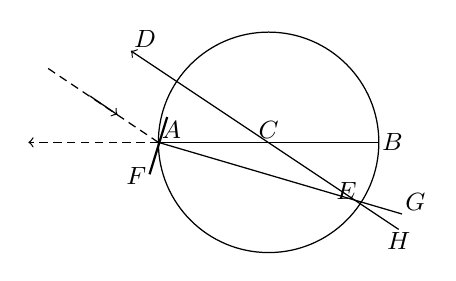
\begin{tikzpicture}[x=14mm,y=14mm,line width=.45pt,every node/.style={font=\small,inner sep=1pt}]
\draw (0,0) circle (1);
\draw (-1,0)--(1,0);
\draw[<-] (-1.25,.83)--(1.18,-.79);
\draw (-1,0)--(1.21,-.65);
\draw[line width=.8pt] (-1.08,-.29)--(-.92,.23);
\draw[densely dashed,->] (-1,0)--(-2.18,0);
\draw[densely dashed] (-2,.67)--(-1,0);
\draw[->] (-1.62,.42)--(-1.37,.25);
\node[above right] at (-1.25,.83) {$D$};
\node[above right] at (-1,0) {$A$};
\node[above] at (0,0) {$C$}; \node[right] at (1,0) {$B$};
\node[above left] at (.83,-.55) {$E$};
\node[below left] at (-1.08,-.20) {$F$};
\node[above right] at (1.21,-.65) {$G$};
\node[below] at (1.18,-.79) {$H$};
\end{tikzpicture}
\end{center}
\vfill\noindent\hfill61*

\clearpage
\noindent\makebox[0pt][l]{\fontsize{13}{16}\selectfont 484}\hfill{\small\textbf{REMARKS.\quad HELIOTROPE.}}\hfill\null\par\medskip
\begingroup\small
\noindent when the telescope $HD$ is pointed at the sun, the mirror $F$ will reflect the light in the direction
$CA$. To bring the object to which light is to be sent into this direction, the instrument, whose horizontal
axis $AB$ is supported by a column rising from a tripod, is set up so that the object appears in the
telescope $HD$ when the latter is parallel to the axis $BA$.
To keep the mirror from obstructing this observation, it was fastened to a ring.

In 1821 \textsc{Gauss} had only one heliotrope in use (cf.\ pp.~349 and 390), in 1822 and 1823 he had 3 each
year (cf.\ pp.~355 and 470), and in 1824 and 1825 he had 4 each year (according to the work reports).
To operate them, in addition to the three regular assistants for the arc measurement (\textsc{Müller}, \textsc{Hartmann} and
\textsc{J.~Gauss}), he had two others at his disposal in 1824 (the student \textsc{Klüver}, who was supplied by the city of Bremen,
and the student \textsc{Baumann}), and only one assistant (\textsc{Klüver}) in 1825.
\par\hfill\textsc{Krüger.}\par\endgroup
\vspace{20mm}
\begin{center}\rule{40mm}{.4pt}\end{center}

\clearpage
\vspace*{40mm}
\begin{center}{\Large\bfseries MEASUREMENT ERRORS.}\end{center}
\clearpage\null\clearpage
\vspace*{14mm}
\begin{center}
{\Large\bfseries POSTHUMOUS PAPERS AND CORRESPONDENCE.}\par\vspace{10mm}
[On the instruments required for the country's triangulation.]
\end{center}
.\ .\ .\ .\ .\ .\ In an extensive trigonometrical survey, instruments of different ranks
for measuring angles indeed have to be used for the various operations. The rank
is determined by the greater or lesser precision attainable with each instrument,
which depends less on the degree of perfection of its workmanship than on the
dimensions of the instrument. Many gradations might be made here, but I limit
myself to a ranking in 3 classes.

The theodolites of 12 inches diameter made in Munich can be used for the
finest angular measurements on the Earth. I assign to the second rank the
repeating theodolites of 8 inches diameter from the \textsc{Reichenbach-Ertel}
workshop. These serve for secondary measurements. For still more subordinate
measurements and for reconnaissance, still smaller theodolites of the third
rank suffice, and if need be the repetitions can be omitted.

A theodolite of the first rank \textls[120]{could} indeed be used for
\textls[120]{all} operations, even subordinate ones. The reason this is not generally done is partly
to spare the larger instruments, partly because they are by nature more
difficult to transport and require far more preparations when set up.

In the arc measurement proper, which initially served a purely scientific
purpose, I used only one first-rank theodolite and a
